\lvli{Confronto tra D-Wave e computer classico}

\lvlii{Definizione di quantum speedup}
L'interesse nei quantum computer è legato alla loro capacità di essere molto più veloci dei computer tradizionali a risolvere un determinato tipo di problemi, questa capacità prende il nome di \idx{quantum speedup}; a livello matematico è possibile definirlo\cite{DDQS} come il limite del rapporto
$$S = \lim_{N \to \infty} \frac{C(N)}{Q(N)}$$
tra il tempo $C(N)$ necessario per un computer classico a risolvere un problema di dimensioni $N$ e $Q(N)$ il tempo per un computer quantistico per risolvere lo stesso problema. Questa definizione non richiede la capacità di un quantum computer di ridurre un problema da esponenziale a polinomiale come anticipato nell'introduziome ma valuta solo la capacità di scaling con l'aumentare delle dimensioni delle complicazioni.


\lvlii{Simulazione del computer quantistico attraverso algoritmi classici}
Per analizzare il quantum speedup del D-Wave è stato scelto di confrontarlo con due algoritmi classici molto simili SA e SQA, nella ricerca del ground state attraverso un modello di Ising a due dimensioni dello spin glass.
Questa scelta è dipesa dalla capacità di essere rimappato in un qualsiasi altro problema np-hard. Per il calcolo di $Q(N)$ sono state fatte delle simulazioni modificando vari parametri nel D-Wave One e nel D-Wave Two e i loro tempi sono stati valutati come $T_{DW}(N) = Q(N)$. Per quanto riguarda i computer classici sono state eseguite delle simulazioni per ogni $C(N)$ le cui prestazioni sono state misurate compensando la componente parallela\cite{EQA} come
 $\frac{T_{SA-SQA}(N)}{N} \simeq C(N)$. Da qui è stata definita\cite{DDQS} la relazione:
$$S_{DW} = \lim_{N \to \infty} \frac{T_{SA-SQA}(N)}{N \cdot T_{DW}(N)}$$

I primi test di comparazione sono stati eseguiti misurando la probabilità di successo $P(s)$ nel trovare il ground state $P(s) = \frac{M_{GS}}{M}$. Per ogni dimensione da $N=8$ a $N=108$ sono stati generati $Q=1000$ problemi casuali, e per ogni problema sono state eseguite $M=1000$ istanze di test.

\begin{figure}[htbp]
  \centering
  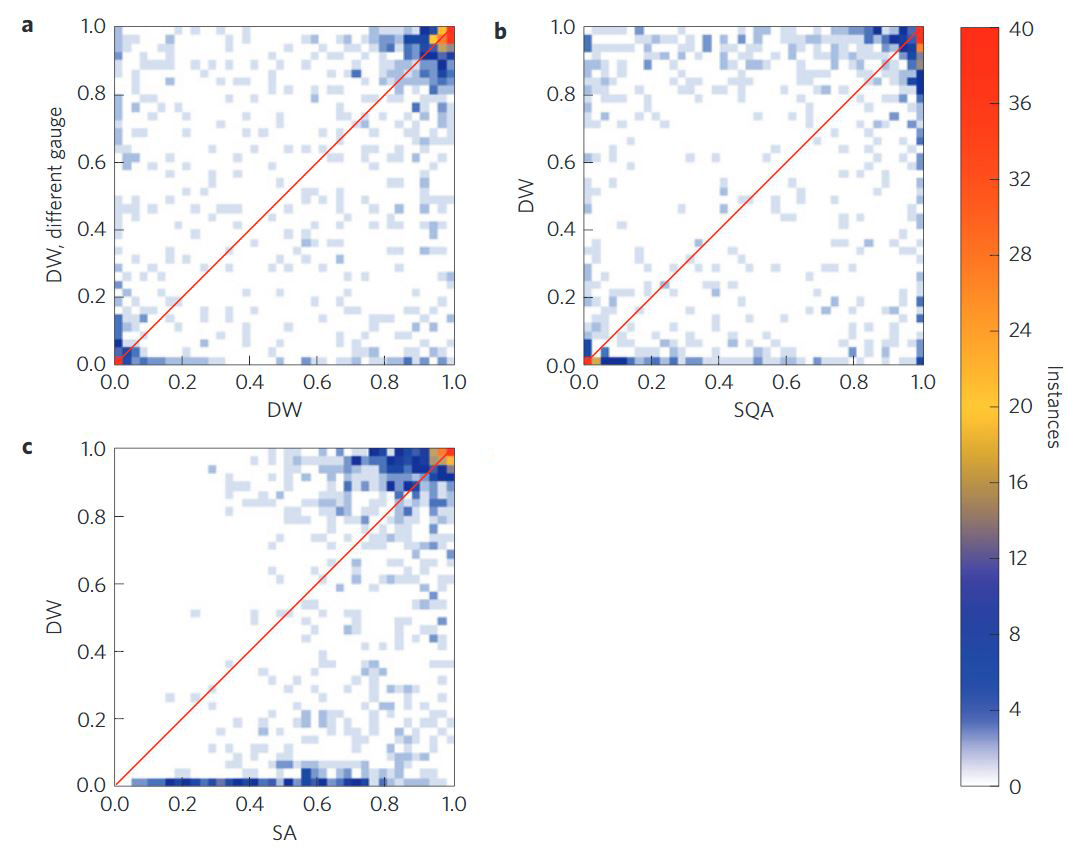
\includegraphics[scale=0.5]{Immagini/correlazione-dw.jpg}
  \caption{Correlazione delle prestazione del DW con gli algoritmi classici.}
  \label{figura:correlazione-dw}
\end{figure}

I risulati sono stati riportati nella figura \ref{figura:correlazione-dw}. Nel primo grafico (a) è messo in mostra la differenza di probabilità di successo tra due configurazioni differenti di parametri impostate sulla stessa macchina della DW per eseguire gli stessi problemi. Nel secondo grafico (b) viene confrontata la macchina DW con il SQA mentre nel terzo grafico (c) sempre la macchina DW ma con il SA. Quello che mettono in mostra questi grafici è che il comportamento della macchina DW è molto più simile al SQA che al SA deducibile dalla presenza di una distribuzione bimodale, visibile all'estremità della linea rossa rappresentante la perfetta correlazione, sia per il DW che per il SQA ma non presente nel SA.


Sono state fatte delle comparazioni tra SA e DW\cite{DDQS} e tra i vari SQA e DW\cite{QVC}, ognuna delle quali ha dimostrato che il DW dopo un certo numero $N_{crit}$ di spin inizia ad avere prestazioni inferiori rispetto ad entrambi gli algoritmi, e ciò denota un'evidente prova della \idx{mancanza di speedup} ad oggi dei sistemi testati. L'assenza di speedup non vuol dire che l'architettura così pensata non possa presentare speedup in futuro, infatti gli ottimi risultati ottenuti dal DW sotto $N_{crit}$ fanno pensare che il quantum speedup non sia raggiunto a causa della difficile calibrazione e rimozione dei rumori termici per grandi $N$ come spiegato nel capitolo dell'architettura.

\lvlii{Confronto tra algoritmi classici}
Nonostante il fallimento nel dimostrare lo speedup si è scoperto un'altro legame molto interessante, quello tra il SQA e il DW. Tale algoritmo approssima bene il comportamento per $N$ molto piccoli e per $N$ molto grandi\cite{EQA}, in particolare la sua versione continua CT-SQA\cite{QVC}. Infatti confermato dalle basi teoriche, solo il CT-SQA è un vero simulatore per il QA perché le approssimazioni utilizzate per il cambiamento da modello quantistico a classico sono fatte considerando evoluzioni continue del sistema.

Il CT-SQA si è rivelato avere prestazioni molto inferiori rispetto al DT-SQA visto che il calcolo usato per ottenerlo attraverso la media delle energie, introduce un'energia residua. Questa osservazione potrebbe essere anche il sintomo che il QA non riesca mai a raggiungere le prestazioni del DT-SQA per colpa proprio di energie residue dovute alla continuità e non dall'effetto termico.

\begin{figure}[htbp]
  \centering
  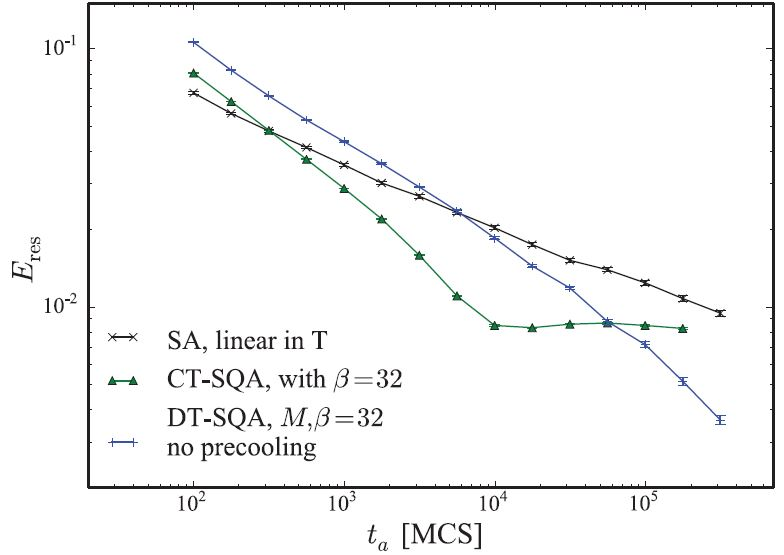
\includegraphics[scale=0.6]{Immagini/residua.jpg}
  \caption{Energie residue nell'esecuzione degli algoritmi.}
  \label{figura:residua}
\end{figure}

\lvlii{Conclusioni}
In conclusione è possibile che in futuro la D-Wave possa ottimizzare il QA in modo tale che presenti uno speed-up rispetto al CT-SQA ma che non sia sufficiente a superare le prestazioni del DT-SQA che si è rivelato essere un ottimo algoritmo per i computer tradizionali. Tutti gli esperimenti realizzati fino ad ora sono stati eseguiti su un modello di Ising a due dimensioni, con condizioni al contorno periodiche, si augura che con il miglioramento dell'architettura del DW sia possibile confrontare modelli a tre dimensioni o superiori e che possano avere risultati differenti.
